\section{PDF Parsing}
\label{sec:parsing}

%%%%% Trust Chain subsection %%%%
\subsection{Data Dependencies in PDF Parsing (the Trust Chain)}
\label{sec:trust-chain}

\begin{figure}[t]
  \centering
  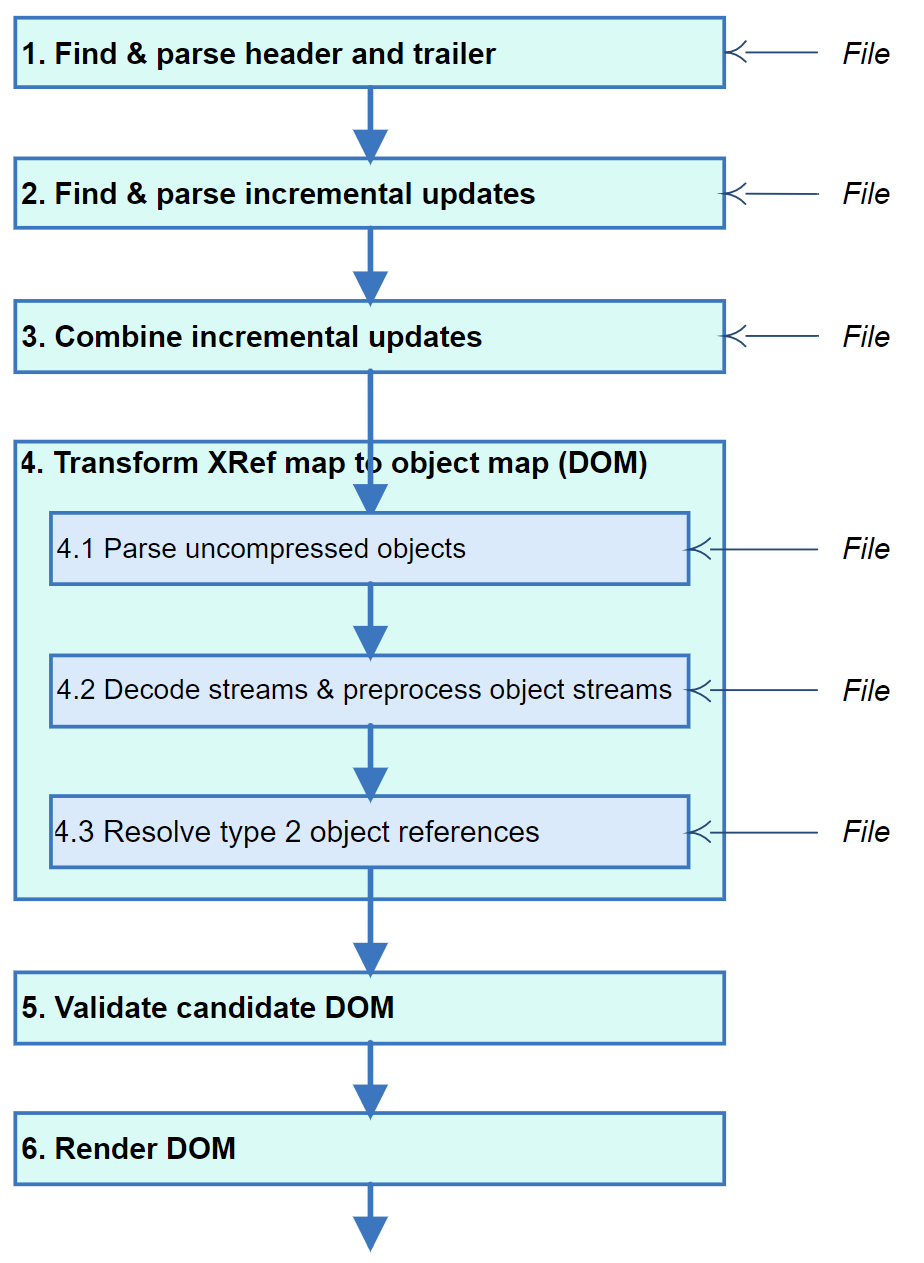
\includegraphics[width=0.8\linewidth]{figures/Stages.png}
  \caption{Stages of PDF Parsing (the Trust Chain)}
  \label{fig:pdf-trust-chain}
\end{figure}

We have touched upon the complexities of parsing
PDF, but to appreciate these, one has to understand the
dependencies and interactions between the features.
\cref{fig:pdf-trust-chain} illustrates the main stages diagrammatically:

\begin{itemize}
\item Stage 1: Find and parse both the PDF header and the PDF trailer to locate
  the document trailer dictionary and the start of the \emph{last} incremental update, or
  the cross reference table of the original document in the case of no updates.
\item Stage 2: Find and parse each cross reference table or incremental update. 
  Note that this stage uses context from Stage 1 (such as the file offset and trailer
  information) in order to know \emph{where} and \emph{how} to parse.
\item Stage 3: This stage computes the
   XRef map of the final PDF by accounting for each set of edits performed by each incremental update.
   Incremental updates can add new objects, mark as free previous objects, re-instate previously 
   freed objects, and change context information in the trailer dictionary that 
   forms part of each incremental update.
   Depending on the laziness of stage 2, this stage may need to do further
   reading of the input file.
\item Stage 4: Transform the XRef map to an object map. This stage is complex and
  requires three sub-stages, each of which does further file input and parsing.
  Further details are in \cref{sec:specifying}.
  If all goes well, we have a syntactically valid candidate DOM.
\item Stage 5: Validate candidate DOM.  This stage takes the candidate DOM and
  \emph{semantically} verifies that it represents a sensible document graph per
  the PDF standard.
  %
  The candidate DOM consists of a mapping of object references to
  syntactically valid PDF objects.  
  Only at this point can we start the semantic checks such as
  dictionaries have the right keys,
  keys have values of the expected types,
  text stream objects are syntactically valid,
  no unexpected recursion, no unresolvable object references,
  and etc.
\item Stage 6: Render the validated DOM. Here the validated DOM, or parts thereof, is rendered
  to the output format of choice.
\end{itemize}

Any error (malicious or otherwise) in an earlier stage will affect the output of stages that follow.
Note that stages 2, 3, 4.1, 4.2, and 4.3 all depend on inputs from previous stages to determine 
where and how to parse segments of the PDF input file.
Errors that percolate into these stages can
cause all forms of havoc (parsing wrong or out-dated data, etc.).

An implementation \emph{might} merge stages 2, 3, 4.1, 4.2, 4.3 into
a single stage and give a \emph{semblance} of simplicity.
%
Our argument in what follows---particularly in
\cref{sec:single-pass-problems}---is
that such an implementation will be overly
complex and result in a design for which it is difficult
to determine if it correctly implements the standard
and to determine that it terminates for all input files.

\todo{cut the following down?:}
Although \emph{Validate candidate DOM} (stage 5) might be considered tedious, the necessary checks are 
reasonably well defined by the bulk of the PDF Standard. Validation involves ensuring that each 
individual PDF object has all the required keys and appropriate values in the context of its reference in the DOM.
For example, a PDF object that is a thumbnail for a PDF page needs to be an Image XObject and have a 
minimum set of required key names and their values each within predefined limits (e.g. both
\lstcd{Height} and \lstcd{Width} are required keys and must be non-negative integers). If the 
thumbnail reference in the candidate DOM is to a font dictionary or some other kind of
\emph{syntactically} valid PDF object then this is \emph{semantically} incorrect. Recent work~
\cite{peterwyattArlingtonPDFModel2021} created the first specification-derived comprehensive
machine-readable model of every object, their attributes and relationships in the PDF DOM. The use
of such a model for code generation, DOM validation, or test case generation can significantly reduce the tediousness.
\emph{Render DOM} (stage 6) also has many complications of its own,
whether this be rendering a PDF
page to pixels for display or print, or extracting text contract.

In this paper we do not further consider stages 5 and 6 but
focus on stages 1 to 4, referred to as \emph{pre-DOM} parsing or computation.
%
Errors in these stages can compromise the correctness of the complete format
definition, even if later stages are defined as intended when viewed in
isolation.

%%%%%%%%%%%%%

The term \emph{Trust Chain} (or ``Chain of Trust'') is
overloaded with similar meanings in different contexts
\begin{quote}
e.g.,
\emph{digital certificates}: a sequence of certificates signing certificates,
starting with a root certificate;
\emph{supply chain}: a product is no more reliable or secure than its
outsourced components;
\emph{trusted boot}: unless the bootloader is correct and non-malicious,
there can be no possibility of the operating system being the same;
\emph{software stacks}: upper layers are dependent upon lower layers (such as
system libraries) and vulnerabilities at the lower layers affect all higher
layers,
\end{quote}
but the common idea is that we have layers (or components)
that rely on lower layers (sub-components) for their validity.
In other words,
{\bf{A flaw in one layer of the trust chain
     causes every higher layer to be untrustworthy!}}

%%%%%%%%%%%%%

Whether or not one likes our adoption of this term,
we think it is important to understand PDF parsing in terms of the
\emph{Trust Chain} principle because
%
(1) it highlights the presence of the many ``dependent'' stages
in PDF processing;
%
(2) it highlights the importance of ensuring the pre-DOM parsing, data integrity relationships and
computation (the base of our Trust Chain) is correct and secure;
%
(3) it reminds us that the integrity of the DOM cannot be verified
independently of verifying all the earlier stages; and
%
(4) it illustrates that PDF parsing, although uniquely complex, is an instance of
a general concept.

 

%%%%%%%%%%%%%%%%%%%%%%%%%%%%%%%%%%%
\subsection{Parsing PDF: More detail}
\label{sec:parsingfile}

We described the physical structure of a PDF file in \Cref{sec:pdf},
but the processing sequence may not be so apparent.
The following paragraphs describe the processing necessary to correctly parse a PDF file containingg incremental updates.

PDF parsing begins by locating the PDF Header, as it is not uncommon for PDF files to have 
preamble bytes (such as an HTTP header, HTML or XML). The offset to the start of the PDF file 
(PDF offset zero)
within a physical file can then be determined from the \lstcd{\%} sign in \lstcd{\%PDF-x.y}. 
Processing continues by seeking to end-of-file and locating the last end-of-file marker \lstcd{\%\%EOF} in the physical file.

It is then necessary to locate the \emph{last} \lstcd{startxref} keyword and the following PDF file byte offset 
to the last cross-reference table in the PDF. Note also that this requires parsing \emph{backwards}
which is unnatural for many programming languages and is a proven source of parser differentials. 
This PDF byte offset must also be adjusted to a physical file offset by accounting for any preamble bytes prior to the PDF Header.

The parsing sublanguage depends on the form of the incremental update, with
conventional cross-reference tables being simpler and largely independent of
other processing. Cross-reference streams however are more complex as they are
often compressed and thus require the pre-DOM parser to ``trust'' the stream
extent dictionary data.

The parser must then locate either the \lstcd{xref} keyword for
conventional PDF cross-reference tables, or a cross-reference stream, identified by tokens of the form \lstcd{x y obj} . 
A parser must then determine if the PDF object is a
semantically valid cross-reference stream by further parsing the stream extent dictionary and 
validating the necessary key/value pairs and also recognizing the \lstcd{stream} keyword after the dictionary end token \lstcd{>>} and the \lstcd{endstream} keyword (see \cref{fig:XRefStm}). 

In the case of conventional PDF
cross-reference tables, after the cross reference table will be the
trailer dictionary, identified by the \lstcd{trailer} keyword. 
Note that this algorithm is at
odds with the file structure as defined in the PDF standard: the Trailer section is formally defined
to contain the trailer dictionary and \lstcd{startxref} keyword, yet the parsing algorithm
requires locating the first trailer \emph{after} the end of the cross-reference table 
(versus the last trailer dictionary above the \lstcd{startxref} keyword). 
Alternatively for PDF 1.5 and later files with cross-reference
streams, the trailer dictionary data will be in the stream extent
dictionary of the cross reference stream. 

Any previous cross-reference data is identified by the value of the \lstcd{/Prev} entry in either
the trailer dictionary or the stream extent dictionary of a cross-reference stream. The
value of the \lstcd{/Prev} key the byte offset to the immediately
preceding cross-reference data which, again, can either be a conventional
cross-reference table and to the start of the \lstcd{xref} keyword, or to a
cross-reference stream. This process repeats, working from the most recent incremental
update back through time to the original PDF document.

In each incremental update, the trailer dictionary is required to duplicate all keys from the previous
trailer and update accordingly. Of particular note is the \lstcd{/Size} entry, which must be
one greater than the largest object number allocated in the PDF file. Objects with numbers greater
than \lstcd{/Size} are defined to be the special PDF \lstcd{null} object.

Data in each cross reference table must be parsed to
identify the byte offset to the start of each PDF object, whether this be a file offset to an indirect object in a Body section, or a relative object position within an object stream (and where the object position is transformed to a byte offset within the object stream from the first line of text in the object stream). Note also that with conventional PDF cross-reference tables there is no definition for the byte offset to the end of an object, however for cross-reference streams this can be pre-determined.

%%%%%%%%%%%%%%%%%%%%%%%%%%%

\subsection{Specifications: Parsing not Recognizing}
\label{sec:spec-approach}

\todo{rewrite! bring in slides}

A useful format specification must resolve a fundamental conflict between precision and restrictiveness.
%
An overly permissive specification, specifically of the PDF pre-DOM,  would permit multiple compliant processors to produce radically different results, and thus would provide little ultimate assurance to format users.
%
Conversely, a specification that formalized all aspects of the standard related to pre-DOM components would prohibit almost all practical document processors, which almost never need to fully validate a document.

% our solution:
To resolve this conflict, we have %
\textbf{(1)} specified an implementation to be as \emph{lazy} as possible, in the sense that it minimizes the data read and validated whenever possible; and %
\textbf{(2)} extended this specification
with separate \lstcd{validate} predicates that, when executed,
would extend our implementation to form a complete validator.
%
Because no implementations validate documents fully, and some implementations
are surprisingly lazy, we want our specification to be very lazy.
%
Due to various redundancies in PDF, there is no one exact
laziest semantics, but we attempt to create something reasonable.
%
The lazier we make our spec (while remaining correct), the more
possible implementations we can test with respect to the spec.
%
We test by validating that the specification's DOM is equivalent to the implementation's DOM,
we don't want to fail in comparison to a tool that gives results when we don't.

% % introduce formal specification:
% We say that a specification is \emph{formal} if it is expressed in a languag% e whose semantics is amenable to a mechanizable definition.
% %
% By their nature, such definitions can offer precision of meaning that is a s% ignificant departure from standards expressed purely in prose;
% %
% in particular, they can provide a basic assurance that they do not rely on u% ndefined terms.
% %
% While their existence does not immediately solve all of the above issues in % format design, they are valuable artifacts for clarifying
% standards, understanding vulnerabilities, and aiding implementors.






